\documentclass[11pt,a4paper]{article}
\usepackage[margin=22mm]{geometry}
\usepackage[T1]{fontenc}
\usepackage{lmodern,amsmath,amssymb,booktabs,array,graphicx}
\usepackage{tikz}
\usetikzlibrary{arrows.meta,calc,positioning,shapes.geometric}
\usepackage[font=small,labelfont=bf]{caption}
\captionsetup{hypcap=false}
\usepackage{enumitem}
\usepackage{microtype}
\usepackage{hyperref}
\definecolor{xc}{HTML}{C45C43}
\definecolor{zc}{HTML}{247F79}
\definecolor{ink}{HTML}{243344}
\hypersetup{colorlinks=true,linkcolor=ink,urlcolor=zc,citecolor=zc}
\setlength{\parindent}{0pt}
\setlength{\parskip}{6pt}
\setlist{nosep,leftmargin=*}
\newcommand{\ket}[1]{\lvert #1\rangle}
\newcommand{\bra}[1]{\langle #1\rvert}
\newcommand{\XL}{\overline{X}}
\newcommand{\ZL}{\overline{Z}}
\newcommand{\SL}{\mathcal{S}}
% Original editable TikZ figures. Coordinates and Pauli supports are checked by
% validate.py. X = orange; Z = teal throughout, including ZX spiders.
\tikzset{data/.style={circle,fill=ink,inner sep=1.6pt},
  zs/.style={circle,draw=zc,fill=zc!30,minimum size=6mm,inner sep=0pt},
  xs/.style={circle,draw=xc,fill=xc!30,minimum size=6mm,inner sep=0pt},
  wire/.style={thick,draw=ink},event/.style={circle,fill=ink,inner sep=2.2pt}}

% d odd; square data grid 0,...,d-1. Even bulk faces X, odd Z.
\newcommand{\rotpatch}[2]{%
\pgfmathtruncatemacro{\dm}{#1-1}
\pgfmathtruncatemacro{\df}{#1-2}
\foreach \x in {0,...,\df}{\foreach \y in {0,...,\df}{
 \pgfmathtruncatemacro{\parity}{mod(\x+\y,2)}
 \ifnum\parity=0 \def\col{xc}\def\typ{X}\else\def\col{zc}\def\typ{Z}\fi
 \filldraw[fill=\col!15,draw=\col!45] (\x,\y) rectangle +(1,1);
 \node[text=\col,font=\scriptsize] at (\x+.5,\y+.5) {$\typ$};
}}
\foreach \i in {0,...,\df}{
 \pgfmathtruncatemacro{\parity}{mod(\i,2)}
 \ifnum\parity=0
  \filldraw[fill=zc!15,draw=zc!45] (\i,0)--(\i+.5,-.45)--(\i+1,0)--cycle;
  \node[text=zc,font=\tiny] at (\i+.5,-.17) {$Z$};
  \filldraw[fill=xc!15,draw=xc!45] (\dm,\i)--(\dm+.45,\i+.5)--(\dm,\i+1)--cycle;
  \node[text=xc,font=\tiny] at (\dm+.17,\i+.5) {$X$};
 \else
  \filldraw[fill=zc!15,draw=zc!45] (\i,\dm)--(\i+.5,\dm+.45)--(\i+1,\dm)--cycle;
  \node[text=zc,font=\tiny] at (\i+.5,\dm+.17) {$Z$};
  \filldraw[fill=xc!15,draw=xc!45] (0,\i)--(-.45,\i+.5)--(0,\i+1)--cycle;
  \node[text=xc,font=\tiny] at (-.17,\i+.5) {$X$};
 \fi
}
\foreach \x in {0,...,\dm}{\foreach \y in {0,...,\dm}{
 \node[data] at (\x,\y) {};
 \ifnum#2=1
  \pgfmathtruncatemacro{\qid}{#1*\y+\x}
  \node[font=\tiny,anchor=south west,fill=white,inner sep=.3pt] at (\x+.035,\y+.035) {\qid};
 \fi
}}
}

\newcommand{\layoutcomparison}{%
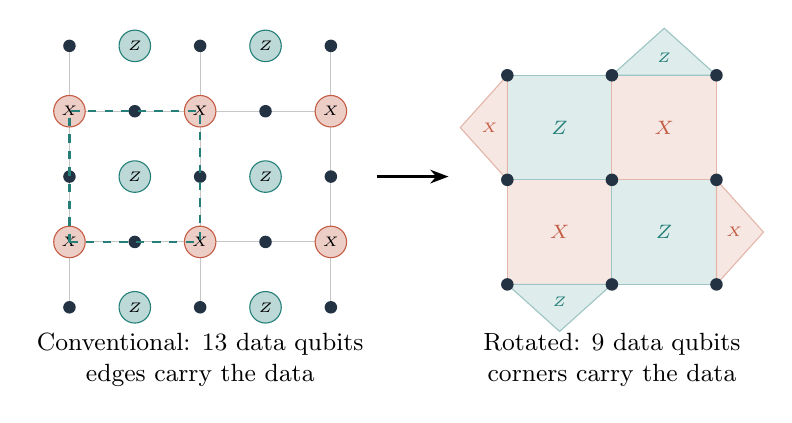
\begin{tikzpicture}[scale=.83]
\begin{scope}
\foreach \x in {0,2,4}{\draw[gray!45] (\x,0)--(\x,4);}
\foreach \y in {1,3}{\draw[gray!45] (0,\y)--(4,\y);}
\foreach \x in {0,...,4}{\foreach \y in {0,...,4}{
 \pgfmathtruncatemacro{\p}{mod(\x+\y,2)}
 \ifnum\p=0 \node[data] at (\x,\y) {};
 \else
  \pgfmathtruncatemacro{\q}{mod(\x,2)}
  \ifnum\q=0 \node[xs,minimum size=4mm,font=\tiny] at (\x,\y) {$X$};
  \else \node[zs,minimum size=4mm,font=\tiny] at (\x,\y) {$Z$};\fi
 \fi
}}
\draw[zc,thick,dashed] (0,1)--(2,1)--(2,3)--(0,3)--cycle;
\node[font=\small,align=center] at (2,-.8) {Conventional: 13 data qubits\\edges carry the data};
\end{scope}
\draw[-{Stealth},thick] (4.7,2)--(5.8,2);
\begin{scope}[shift={(6.7,.35)},scale=1.6]
\rotpatch{3}{0}
\end{scope}
\node[font=\small,align=center] at (8.3,-.8) {Rotated: 9 data qubits\\corners carry the data};
\end{tikzpicture}}

\newcommand{\detailedpatch}{%
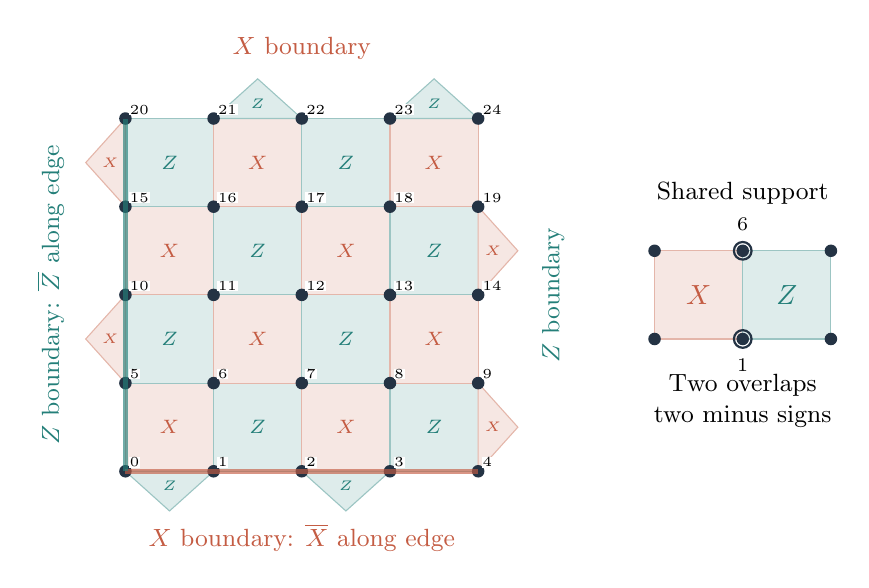
\begin{tikzpicture}[scale=1.12]
\rotpatch{5}{1}
\draw[xc,line width=2pt,opacity=.65] (0,0)--(4,0);
\draw[zc,line width=2pt,opacity=.65] (0,0)--(0,4);
\node[text=xc,font=\small] at (2,4.8) {$X$ boundary};
\node[text=xc,font=\small] at (2,-.75) {$X$ boundary: $\XL$ along edge};
\node[text=zc,rotate=90,font=\small] at (-.85,2) {$Z$ boundary: $\ZL$ along edge};
\node[text=zc,rotate=90,font=\small] at (4.85,2) {$Z$ boundary};
\begin{scope}[shift={(6,1.5)}]
\filldraw[fill=xc!15,draw=xc!45] (0,0) rectangle (1,1);
\filldraw[fill=zc!15,draw=zc!45] (1,0) rectangle (2,1);
\node[text=xc] at (.5,.5) {$X$};\node[text=zc] at (1.5,.5) {$Z$};
\foreach \x in {0,1,2}{\foreach \y in {0,1}{\node[data] at (\x,\y) {};}}
\draw[ink,thick] (1,0) circle (.1) (1,1) circle (.1);
\node[font=\scriptsize,anchor=north] at (1,-.12) {1};
\node[font=\scriptsize,anchor=south] at (1,1.12) {6};
\node[font=\small] at (1,1.65) {Shared support};
\node[font=\small,align=center] at (1,-.7) {Two overlaps\\two minus signs};
\end{scope}
\end{tikzpicture}}

\newcommand{\schedules}{%
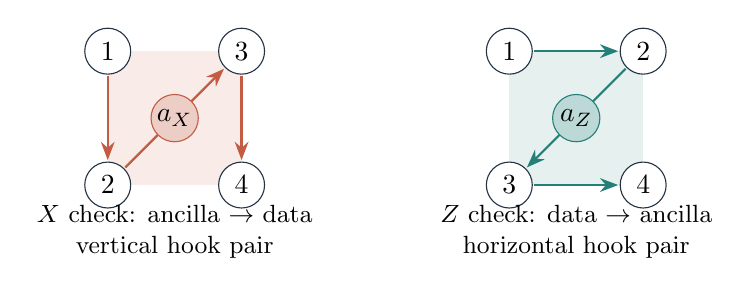
\begin{tikzpicture}[scale=.85]
\begin{scope}
\fill[xc!12] (0,0) rectangle (2,2);
\draw[xc,thick,-{Stealth},shorten <=9pt,shorten >=9pt] (0,2)--(0,0);
\draw[xc,thick,-{Stealth},shorten <=9pt,shorten >=9pt] (0,0)--(2,2);
\draw[xc,thick,-{Stealth},shorten <=9pt,shorten >=9pt] (2,2)--(2,0);
\node[xs] at (1,1) {$a_X$};
\foreach \x/\y/\n in {0/2/1,0/0/2,2/2/3,2/0/4}{\node[circle,fill=white,draw=ink,inner sep=3pt] at (\x,\y) {\n};}
\node[font=\small,align=center] at (1,-.7) {$X$ check: ancilla $\to$ data\\vertical hook pair};
\end{scope}
\begin{scope}[xshift=6cm]
\fill[zc!12] (0,0) rectangle (2,2);
\draw[zc,thick,-{Stealth},shorten <=9pt,shorten >=9pt] (0,2)--(2,2);
\draw[zc,thick,-{Stealth},shorten <=9pt,shorten >=9pt] (2,2)--(0,0);
\draw[zc,thick,-{Stealth},shorten <=9pt,shorten >=9pt] (0,0)--(2,0);
\node[zs] at (1,1) {$a_Z$};
\foreach \x/\y/\n in {0/2/1,2/2/2,0/0/3,2/0/4}{\node[circle,fill=white,draw=ink,inner sep=3pt] at (\x,\y) {\n};}
\node[font=\small,align=center] at (1,-.7) {$Z$ check: data $\to$ ancilla\\horizontal hook pair};
\end{scope}
\end{tikzpicture}}

\newcommand{\errorpatch}{%
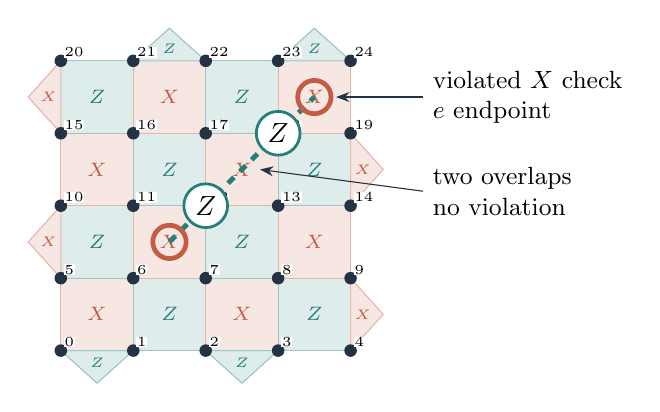
\begin{tikzpicture}[scale=.92]
\rotpatch{5}{1}
\draw[zc,line width=1.8pt,dashed] (1.5,1.5)--(3.5,3.5);
\foreach \p in {(2,2),(3,3)}{\node[circle,draw=zc,fill=white,line width=1pt,inner sep=2pt] at \p {$Z$};}
\foreach \p in {(1.5,1.5),(3.5,3.5)}{\draw[xc,line width=1.7pt] \p circle (.23);}
\draw[-{Stealth},ink] (5,3.5)--(3.8,3.5);
\node[anchor=west,font=\small,align=left] at (5,3.5) {violated $X$ check\\$e$ endpoint};
\draw[-{Stealth},ink] (5,2.2)--(2.75,2.5);
\node[anchor=west,font=\small,align=left] at (5,2.2) {two overlaps\\no violation};
\end{tikzpicture}}

% Abstract square: horizontal X edges, vertical Z edges.
\newcommand{\squarepatch}[1][1]{%
\fill[ink!3] (0,0) rectangle (2,2);
\draw[xc,line width=2pt] (0,0)--(2,0) (0,2)--(2,2);
\draw[zc,line width=2pt] (0,0)--(0,2) (2,0)--(2,2);
\ifnum#1=1
\node[text=xc,font=\scriptsize] at (1,2.2) {$X$};
\node[text=xc,font=\scriptsize] at (1,-.2) {$X$};
\node[text=zc,font=\scriptsize] at (-.2,1) {$Z$};
\node[text=zc,font=\scriptsize] at (2.2,1) {$Z$};\fi}

\newcommand{\abstractstrings}{%
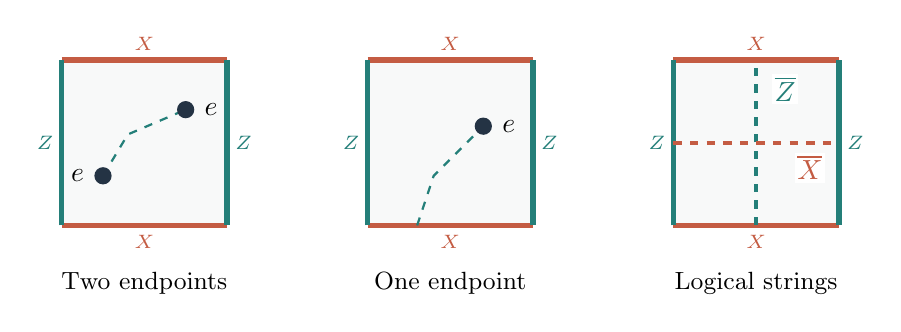
\begin{tikzpicture}[scale=1.05]
\squarepatch
\draw[zc,thick,dashed] (.5,.6)--(.8,1.1)--(1.5,1.4);
\node[event,label=left:$e$] at (.5,.6) {};
\node[event,label=right:$e$] at (1.5,1.4) {};
\node[font=\small] at (1,-.7) {Two endpoints};
\begin{scope}[xshift=3.7cm]
\squarepatch
\draw[zc,thick,dashed] (.6,0)--(.8,.6)--(1.4,1.2);
\node[event,label=right:$e$] at (1.4,1.2) {};
\node[font=\small] at (1,-.7) {One endpoint};
\end{scope}
\begin{scope}[xshift=7.4cm]
\squarepatch
\draw[zc,line width=1.5pt,dashed] (1,0)--(1,2);
\draw[xc,line width=1.5pt,dashed] (0,1)--(2,1);
\node[fill=white,inner sep=1pt,text=zc] at (1.35,1.65) {$\ZL$};
\node[fill=white,inner sep=1pt,text=xc] at (1.65,.7) {$\XL$};
\node[font=\small] at (1,-.7) {Logical strings};
\end{scope}
\end{tikzpicture}}

\newcommand{\memorydiagram}{%
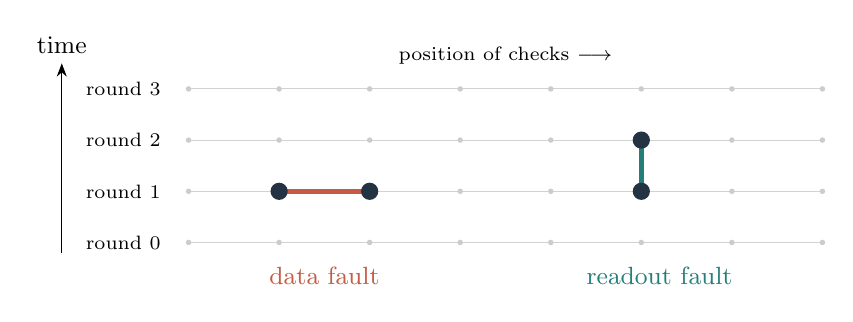
\begin{tikzpicture}[x=1.15cm,y=.65cm]
\foreach \t in {0,1,2,3}{
 \draw[gray!35] (0,\t)--(7,\t);
 \node[anchor=east,font=\scriptsize] at (-.2,\t) {round $\t$};
 \foreach \x in {0,...,7}{\fill[gray!40] (\x,\t) circle (1pt);}
}
\draw[-{Stealth}] (-1.4,-.2)--(-1.4,3.5) node[above,font=\small] {time};
\draw[xc,line width=2pt] (1,1)--(2,1);
\node[event] at (1,1) {};\node[event] at (2,1) {};
\draw[zc,line width=2pt] (5,1)--(5,2);
\node[event] at (5,1) {};\node[event] at (5,2) {};
\node[font=\small,text=xc] at (1.5,-.65) {data fault};
\node[font=\small,text=zc] at (5.2,-.65) {readout fault};
\node[font=\scriptsize] at (3.5,3.65) {position of checks $\longrightarrow$};
\end{tikzpicture}}

\newcommand{\surgerypair}[1]{%
\begin{scope}[scale=.7]
\squarepatch[0]
\begin{scope}[xshift=2.5cm]\squarepatch[0]\end{scope}
\node at (1,1) {$1$};\node at (3.5,1) {$2$};
\ifnum#1=1
\fill[zc!25] (2,-.02) rectangle (2.5,2.02);
\draw[zc,thick] (2,0)--(2.5,0) (2,2)--(2.5,2);
\fi
\end{scope}}
\newcommand{\surgerydiagram}{%
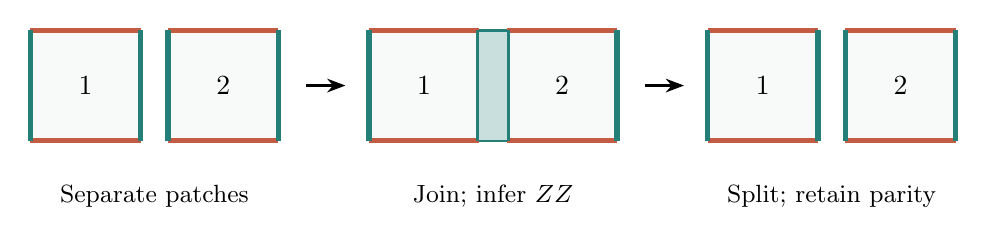
\begin{tikzpicture}
\surgerypair{0}
\node[font=\small] at (1.575,-.7) {Separate patches};
\draw[-{Stealth},thick] (3.5,.7)--(4,.7);
\begin{scope}[xshift=4.3cm]\surgerypair{1}\end{scope}
\node[font=\small] at (5.875,-.7) {Join; infer $ZZ$};
\draw[-{Stealth},thick] (7.8,.7)--(8.3,.7);
\begin{scope}[xshift=8.6cm]\surgerypair{0}\end{scope}
\node[font=\small] at (10.175,-.7) {Split; retain parity};
\end{tikzpicture}}

\newcommand{\cnotstage}[1]{%
\begin{scope}[scale=.55]
\squarepatch[0]\node at (1,1) {$C$};
\begin{scope}[xshift=2.6cm]\squarepatch[0]\node at (1,1) {$A$};\end{scope}
\begin{scope}[shift={(2.6,-2.6)}]\squarepatch[0]\node at (1,1) {$T$};\end{scope}
\ifnum#1=1 \fill[zc!40] (2,0) rectangle (2.6,2);\fi
\ifnum#1=2 \fill[xc!40] (2.6,-.6) rectangle (4.6,0);\fi
\ifnum#1=3 \node[fill=white,font=\small] at (3.6,1) {$Z_A$};\fi
\end{scope}}
\newcommand{\cnotpatches}{%
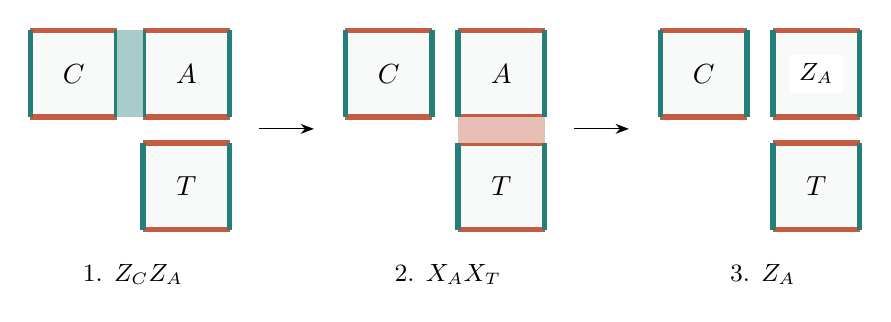
\begin{tikzpicture}
\cnotstage{1}\node[font=\small] at (1.3,-2) {1. $Z_CZ_A$};
\draw[-{Stealth}] (2.9,-.15)--(3.6,-.15);
\begin{scope}[xshift=4cm]\cnotstage{2}\end{scope}
\node[font=\small] at (5.3,-2) {2. $X_AX_T$};
\draw[-{Stealth}] (6.9,-.15)--(7.6,-.15);
\begin{scope}[xshift=8cm]\cnotstage{3}\end{scope}
\node[font=\small] at (9.3,-2) {3. $Z_A$};
\end{tikzpicture}}

\newcommand{\zxdiagram}{%
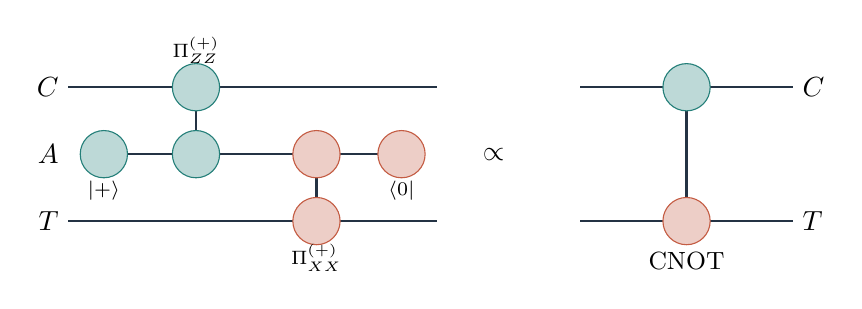
\begin{tikzpicture}[x=.9cm,y=.85cm]
\node[anchor=east] at (0,2) {$C$};
\node[anchor=east] at (0,1) {$A$};
\node[anchor=east] at (0,0) {$T$};
\draw[wire] (0,2)--(5.2,2) (0,0)--(5.2,0) (.5,1)--(4.7,1);
\draw[wire] (1.8,2)--(1.8,1) (3.5,1)--(3.5,0);
\node[zs] at (1.8,2) {};\node[zs] at (1.8,1) {};
\node[xs] at (3.5,1) {};\node[xs] at (3.5,0) {};
\node[zs] at (.5,1) {};\node[xs] at (4.7,1) {};
\node[font=\scriptsize] at (.5,.45) {$\ket{+}$};
\node[font=\scriptsize] at (4.7,.45) {$\bra{0}$};
\node[font=\scriptsize] at (1.8,2.55) {$\Pi_{ZZ}^{(+)}$};
\node[font=\scriptsize] at (3.5,-.55) {$\Pi_{XX}^{(+)}$};
\node at (6,1) {$\propto$};
\begin{scope}[xshift=6.5cm]
\draw[wire] (0,2)--(3,2) (0,0)--(3,0) (1.5,0)--(1.5,2);
\node[zs] at (1.5,2) {};\node[xs] at (1.5,0) {};
\node[font=\small] at (1.5,-.6) {CNOT};
\node[anchor=west] at (3,2) {$C$};\node[anchor=west] at (3,0) {$T$};
\end{scope}
\end{tikzpicture}}

\begin{document}
\begin{center}
{\Large\bfseries Tutorial 2: Rotated Surface Codes}\\[5pt]
{\large From local checks to lattice surgery}
\end{center}

How can we protect quantum information when a device can only couple nearby qubits?

In this tutorial, we arrange stabilizer checks on a lattice, use their geometry to understand errors, and then turn a quantum memory into a logical CNOT. We assume familiarity with Pauli operators, stabilizers, CNOT gates, and the Pauli frame, as introduced in the Shor-code tutorial.

\section{From Shor's code to local checks}

A \textbf{geometrically local code} places qubits in space and uses checks whose support stays within a bounded neighborhood as the code grows. The surface code is a two-dimensional example. Its geometry also makes it a \textbf{topological code}: local checks cannot distinguish the logical states, while certain extended strings act on the encoded information.

The connection to Shor's code is the stabilizer condition:
\[
S_i\ket{\psi_L}=\ket{\psi_L}.
\]
Both codes use separate $X$- and $Z$-type checks, a structure called \textbf{CSS}. We still infer errors from check outcomes without measuring the encoded amplitudes. What changes is the arrangement and support of the checks. The nine-qubit Shor code and the distance-three rotated surface code both have parameters $[[9,1,3]]$, but they have different stabilizer groups.

\subsection*{Why use this geometry?}
Each check couples only a few neighboring qubits. Increasing the patch size increases the minimum size of an undetectable logical Pauli operator, called the \textbf{code distance} $d$. This provides a route to stronger protection without requiring each qubit to connect to more distant neighbors.

Surface codes are used in experiments: repeated error correction and decreasing logical error with increasing distance have been demonstrated under suitable operating conditions~\cite{google}. They are not automatically beneficial at every physical error rate. Performance depends on the noise, measurement circuit, and decoder.

The cost is substantial. A square rotated patch uses $d^2$ data qubits for one logical qubit, plus measurement ancillas. Checks must be repeated, their results decoded, and logical gates require additional space and time. Locality is useful, but it does not make fault tolerance free.

\newpage
\section{Why is it called rotated?}

In the conventional surface-code lattice, data qubits sit on \textbf{edges}. An $X$ check acts on edges meeting at a vertex; a $Z$ check acts around a face. A finite patch has truncated checks at its boundaries.

The rotated construction chooses boundaries at $45^\circ$ to this underlying lattice and removes surplus boundary qubits. After redrawing, the data qubits form a square grid and sit at the \textbf{corners of checkerboard faces}. This changes the patch cut; merely turning a drawing does not change the code~\cite{horsman}.

\begin{center}
\layoutcomparison
\captionof{figure}{Two distance-three patches. Black dots are data qubits; colored markers or faces are checks. The dashed square highlights one $Z$ plaquette in the conventional lattice. The right drawing places data at face corners. Ancillas are excluded from the counts.}
\end{center}

For the usual square patches with the same distance,
\[
n_{\mathrm{conventional}}=d^2+(d-1)^2,
\qquad n_{\mathrm{rotated}}=d^2.
\]
Thus $d=3$ requires 13 or 9 data qubits, respectively. Both patches encode one logical qubit. Rotation saves space while preserving distance; it does not by itself establish a better error rate under every noise model.

\subsection*{Our drawing convention}
Throughout the tutorial, \textcolor{xc}{$X$ checks are orange} and \textcolor{zc}{$Z$ checks are teal}. A black dot is a data qubit. A check region specifies which data qubits participate; a measurement ancilla, when shown, sits near its center.

We label a boundary by the \emph{logical operator supported along it}: the top and bottom are $X$ boundaries, and the left and right are $Z$ boundaries. This is a patch-operator convention, following Litinski's visual representation~\cite{litinski}. It does not name the truncated check at that edge.

\newpage
\section{Reading the checks and boundaries}

For a face $f$, the corresponding stabilizer is
\[
S_X(f)=\prod_{j\in\operatorname{corners}(f)}X_j,
\qquad
S_Z(f)=\prod_{j\in\operatorname{corners}(f)}Z_j.
\]
Bulk checks have weight four; the boundary half-faces have weight two. In Figure~\ref{fig:patch}, qubit $q_{x,y}$ has label $5y+x$.

\begin{center}
\detailedpatch
\captionof{figure}{A distance-five rotated patch: 25 data qubits and 24 independent checks. Letters label check types, not extra data qubits. The paths represent $\XL$ and $\ZL$. The inset isolates the two shared data qubits of the neighboring checks used below.}\label{fig:patch}
\end{center}

For example, neighboring bulk checks are
\[
S_X=X_0X_1X_5X_6,
\qquad S_Z=Z_1Z_2Z_6Z_7.
\]
They overlap at qubits 1 and 6. Each overlap contributes a minus sign when we exchange $X$ and $Z$, so
\[
S_XS_Z=(-1)^2S_ZS_X=S_ZS_X.
\]
Every unlike pair of checks shares zero or two qubits; like-type checks commute automatically. The checks can therefore constrain the state simultaneously.

In contrast, a single $Z_6$ anticommutes with the displayed $X$ check because it overlaps once. Its outcome changes from $+1$ to $-1$. We record $+1$ as syndrome bit 0 and $-1$ as bit 1.

\newpage
\section{Does the measurement order matter?}

The stabilizers commute, so the order of \emph{ideal projective check measurements} does not matter. Their physical implementation is a different question.

To measure a $Z$ check, prepare an ancilla in $\ket{0}$, apply CNOTs from each participating data qubit to the ancilla, and measure the ancilla in $Z$. For an $X$ check, prepare $\ket{+}$, use the ancilla as the CNOT control, and measure it in $X$.

\begin{center}
\schedules
\captionof{figure}{One compatible four-layer bulk schedule for our patch orientation. Numbers give the CNOT interaction layer at each corner; the paths are ordering guides, not data--data gates. Boundary checks omit missing corners while retaining the layer numbers.}
\end{center}

For this orientation, we use an N-shaped order for $X$ checks and a Z-shaped order for $Z$ checks:
\[
\begin{aligned}
X &: \mathrm{NW}\to\mathrm{SW}\to\mathrm{NE}\to\mathrm{SE},\\
Z &: \mathrm{NW}\to\mathrm{NE}\to\mathrm{SW}\to\mathrm{SE}.
\end{aligned}
\]
These are four shared time layers across the patch. The orders must avoid two gates using the same qubit at once and implement compatible parity measurements; independently choosing an order for every face is not sufficient.

\subsection*{Why N and Z?}
A fault on a measurement ancilla can propagate to several data qubits. For example, an $X$ fault on the control ancilla of an $X$ check, after its second CNOT, spreads to its last two targets. The resulting correlated pair is called a \textbf{hook error}.

Here the last two data qubits touched by an $X$ check form a vertical pair, transverse to our horizontal $\XL$. For a $Z$ check, they form a horizontal pair, transverse to our vertical $\ZL$. This prevents these two-qubit hooks from taking a two-site step along the corresponding shortest logical string. Good schedules account for this orientation~\cite{cudaq}.

The letters are drawing mnemonics, not universal rules: rotating the patch or exchanging $X$ and $Z$ changes the appropriate order. A full circuit still needs fault analysis, including preparation, readout, and boundary operations.

\newpage
\section{Errors, strings, and Pauli charges}

An error is a Pauli operator on data qubits; a syndrome is the set of check outcomes it changes. These are different objects. A line in the following pictures represents a \emph{product} of errors along a path, not a particle's measured trajectory.

\begin{center}
\errorpatch
\captionof{figure}{The error $E=Z_{12}Z_{18}$ flips the two circled $X$ checks. The intermediate $X$ check overlaps both error factors, so its outcome is unchanged. The dashed line joins check centers through the affected data qubits.}
\end{center}

We call a violated check an \textbf{endpoint charge}. In the usual anyon language, a violated $X$ check is an $e$ charge, created at an endpoint of a $Z$ string; a violated $Z$ check is an $m$ charge, created by an $X$ string~\cite{kitaev}. These are not electric charges. Here, ``Pauli charge'' refers to this syndrome content of a Pauli string.

Two identical endpoint charges cancel when strings join, because syndromes add modulo two:
\[
\mathbf{s}(E_1E_2)=\mathbf{s}(E_1)\oplus\mathbf{s}(E_2).
\]
A $Y=iXZ$ error combines both kinds of syndrome. In the bulk, a string has two endpoints. At a suitable boundary, one endpoint can disappear without violating a check.

Multiplying an error by a stabilizer changes its physical support without changing its syndrome or action on encoded states. This is why a decoder chooses a \emph{recovery class}, rather than reconstructing a unique history. A recovery $C$ succeeds if $CE\in\SL$, up to global phase. Having zero residual syndrome alone is not enough: $CE$ could still be a logical operator.

\newpage
\section{Zooming out to a logical patch}

We can now hide the microscopic checks and draw one square per logical qubit. This patch view is inspired by \emph{A Game of Surface Codes}~\cite{litinski}; the figures here are original schematics.

\begin{center}
\abstractstrings
\captionof{figure}{Left: a $Z$ string with two detectable $e$ endpoints. Middle: an endpoint is absorbed at an $X$ boundary. Right: $\ZL$ connects the two $X$ boundaries, while $\XL$ connects the two $Z$ boundaries. Neither logical string has a syndrome endpoint.}
\end{center}

The boundary convention is worth making explicit:
\begin{center}
\begin{tabular}{lll}
\toprule
Boundary label & Operator along the edge & String that can end there\\
\midrule
$X$ (top/bottom) & $\XL$ & $Z$ string ($e$ charge)\\
$Z$ (left/right) & $\ZL$ & $X$ string ($m$ charge)\\
\bottomrule
\end{tabular}
\end{center}
With our charge convention, the $X$ boundaries absorb $e$ and are called rough; the $Z$ boundaries absorb $m$ and are called smooth. We use explicit operator and endpoint labels because boundary naming conventions vary between references.

\subsection*{Seeing the logical algebra}
For our numbered patch, choose
\[
\XL=X_0X_1X_2X_3X_4,
\qquad
\ZL=Z_0Z_5Z_{10}Z_{15}Z_{20}.
\]
Both commute with every check, but overlap each other on exactly one qubit:
\[
\XL\ZL=-\ZL\XL.
\]
The crossing in the square is the geometric version of this odd overlap. A shortest nontrivial string contains $d$ data qubits. Contractible closed strings are stabilizers; a string spanning the appropriate opposite boundaries can act on the logical qubit without announcing itself in the syndrome.

The same picture explains decoding failure: the actual error and chosen recovery can join into a spanning logical string even though their endpoints match and cancel.

\newpage
\section{A memory experiment with repeated checks}

How reliably does the patch preserve a logical qubit for $T$ rounds?

\begin{enumerate}
\item \textbf{Prepare.} For a $Z$-basis memory, initialize data in $\ket{0}^{\otimes d^2}$ and establish the checks, recording the initially random $X$-check signs in the frame. For an $X$-basis memory, start with $\ket{+}^{\otimes d^2}$ and exchange $X$ and $Z$.
\item \textbf{Repeat.} Measure checks with ancillas for $T$ rounds. A specified circuit noise model can include data, gate, reset, idle, and measurement faults.
\item \textbf{Decode.} Use the measurement history to infer a recovery and track its Pauli frame.
\item \textbf{Read out.} Measure all data in the chosen basis. Their parities give the final logical measurement and final compatible check values. Include these in decoding before adjusting the logical result.
\end{enumerate}

\begin{center}
\memorydiagram
\captionof{figure}{A slice of a space--time detection graph for one check type. A data fault can join neighboring checks in space. A flipped check readout can join events on the same check in consecutive rounds. Real circuit faults can also create diagonal or more complicated event patterns.}
\end{center}

Let $s_i(t)$ be a check's measured bit in round $t$. Away from initialization and readout, a \textbf{detection event} is
\[
D_i(t)=s_i(t)\oplus s_i(t-1).
\]
A persistent data error changes the syndrome when it occurs; it does not create a new event every round. An isolated wrong readout usually creates events in two neighboring rounds. Initial comparisons use only known preparation constraints; final comparisons use the checks inferable from the data-measurement basis.

For $N$ shots at fixed $d$ and $T$, report
\[
\widehat p_{L,B}(T)=\frac{\text{incorrect frame-adjusted logical readouts in basis }B}{N},
\qquad B\in\{X,Z\}.
\]
These are failure probabilities for the entire experiment, not automatically per-round rates. Run both bases: a $Z$ readout detects logical $X/Y$ errors, while an $X$ readout detects logical $Z/Y$ errors. Numerical performance requires a specified noise model, schedule, and decoder.

\newpage
\section{Lattice surgery: measuring between patches}

A memory preserves one logical qubit. To compute, we also need operations that couple logical qubits. Lattice surgery implements joint logical measurements while retaining local physical interactions~\cite{horsman}.

Suppose two patches share facing $Z$ boundaries. We temporarily replace checks near the interface with compatible checks that join the patches. Products of their outcomes, together with known check and frame signs, reveal $\ZL_1\ZL_2$. Restoring separate patches completes a parity-measurement operation. Facing $X$ boundaries similarly allow $\XL_1\XL_2$.

The measured eigenvalue gives a \emph{relation} between logical values, not either value separately. For example,
\[
\Pi_{ZZ}^{(+)}\ket{+}_L\ket{+}_L
\propto \ket{00}_L+\ket{11}_L,
\qquad
\Pi_{ZZ}^{(+)}=\frac{I+\ZL_1\ZL_2}{2}.
\]
The $-1$ branch instead gives an odd-parity Bell state. The outcome is recorded and its effect tracked.

\begin{center}
\surgerydiagram
\captionof{figure}{A patch-level $ZZ$ measurement. The teal seam joins facing $Z$ edges. ``Join'' means changing and repeatedly measuring interface checks, not directly measuring all data qubits along the seam. The picture omits physical bridge-qubit and gate details.}
\end{center}

\subsection*{Where does the time cost enter?}
One noisy interface measurement is insufficient. In standard distance-$d$ protocols, a surgery stage uses on the order of $d$ syndrome rounds, together with suitable spatial separation, to protect the parity result against measurement faults. Splitting also needs correct frame bookkeeping; separating drawings alone is not a physical protocol.

Lattice surgery is useful when joint logical measurements and entangling gates must respect local connectivity. It is one route to logical computation, not the only one. We will use two such parity measurements to build a CNOT.

\newpage
\section{A CNOT from parity measurements}

Let $C$ and $T$ be arbitrary control and target logical qubits. Prepare an ancillary \emph{logical patch} $A$ in $\ket{+}_L$; this is different from a single physical check ancilla.

Use the following sequence, where outcome bit $m$ denotes eigenvalue $(-1)^m$. In a noisy implementation, $a,b,c$ are decoded logical outcomes, interpreted using the incoming Pauli frame:
\begin{center}
\begin{tabular}{cll}
\toprule
Step & Operation & Outcome\\
\midrule
1 & Measure $\ZL_C\ZL_A$ & $a$\\
2 & Measure $\XL_A\XL_T$ & $b$\\
3 & Measure $\ZL_A$ and discard $A$ & $c$\\
4 & Track $\ZL_C^{\,b}\XL_T^{\,a\oplus c}$ & Pauli frame update\\
\bottomrule
\end{tabular}
\end{center}

\begin{center}
\cnotpatches
\captionof{figure}{An L-shaped layout allows $C$--$A$ to meet on $Z$ edges and $A$--$T$ on $X$ edges. Highlighted seams show successive parity measurements; each stage restores the separate patches before the next. The last stage reads out the ancilla patch.}
\end{center}

\subsection*{Why does this give CNOT?}
For logical computational-basis input $\ket{x}_C\ket{y}_T$, the first measurement fixes the ancilla value to $x\oplus a$. The second creates the two branches related by $X_AX_T$. The final result $c$ selects the target value $y\oplus x\oplus a\oplus c$, with relative phase $(-1)^{bx}$, up to an outcome-dependent global phase.

Thus the uncorrected branch acts as
\[
\ket{\psi}_{CT}\longmapsto
\ZL_C^{\,b}\XL_T^{\,a\oplus c}
\operatorname{CNOT}_{C\to T}\ket{\psi}_{CT},
\]
up to normalization and global phase. The frame update removes those known byproducts in subsequent interpretation. Linearity makes the argument valid for superpositions and entangled inputs, not just basis states.

Unlike memory checks, these two joint observables anticommute on $A$. Their \emph{sequence} is part of the logical protocol and must not be freely reordered.

\newpage
\section{The same operation as a ZX graph}

ZX diagrams describe logical linear maps. Wires are logical systems, and colored nodes, called \textbf{spiders}, represent copying or matching amplitudes in a chosen basis. They are not physical stabilizer faces or endpoint charges.

For zero phase, a $Z$ spider (teal/green) with $m$ inputs and $n$ outputs is
\[
Z_{m,n}=\ket{0}^{\otimes n}\bra{0}^{\otimes m}
+\ket{1}^{\otimes n}\bra{1}^{\otimes m}.
\]
An $X$ spider (orange/red) uses $\ket{+},\ket{-}$ instead. Normalization scalars are often suppressed when drawing a fixed measurement branch. Connected spiders of the same color fuse; a split and merge in the corresponding basis therefore have a compact graphical description~\cite{zx}.

\begin{center}
\zxdiagram
\captionof{figure}{The all-$+1$ branch of the parity-measurement CNOT, reduced to its ZX form. Time runs left to right. A $ZZ$ projector connects two $Z$ spiders; an $XX$ projector connects two $X$ spiders. The one-legged $Z$ preparation is $\ket{+}$ and the one-legged $X$ effect is $\bra{0}$, up to scalars.}
\end{center}

In the left graph, fuse the connected $Z$ spiders, including the $\ket{+}_A$ preparation. Fuse the connected $X$ spiders, including the $\bra{0}_A$ effect. The remaining graph is a $Z$ spider on the control wire joined to an $X$ spider on the target wire: the standard CNOT graph, up to the suppressed scalar.

The other outcome branches have Pauli byproducts. For our measurement convention, these are precisely $\ZL_C^b\XL_T^{a\oplus c}$ from the previous section. A positive-branch graph alone does not describe the deterministic protocol; the outcome record and frame update complete it.

\subsection*{What happened to the charges?}
At the physical level, endpoint charges tell us which local checks an error violates. At the logical level, Pauli propagation tells us how a pending frame moves through the operation:
\[
\begin{aligned}
X_C&\longmapsto X_CX_T, & Z_C&\longmapsto Z_C,\\
X_T&\longmapsto X_T, & Z_T&\longmapsto Z_CZ_T.
\end{aligned}
\]
Here $X_C,Z_C,X_T,Z_T$ denote logical operators. This connects the syndrome-and-frame story to the logical graph without identifying microscopic charges with spiders. The patch diagrams explain \emph{where} the operation can happen; the ZX graph explains \emph{which logical map} it implements.

\newpage
\begin{thebibliography}{9}
\bibitem{horsman} C. Horsman, A. G. Fowler, S. Devitt, and R. Van Meter, \emph{Surface code quantum computing by lattice surgery}, New J. Phys. 14, 123011 (2012). \href{https://arxiv.org/abs/1111.4022}{arXiv:1111.4022}.
\bibitem{litinski} D. Litinski, \emph{A Game of Surface Codes: Large-Scale Quantum Computing with Lattice Surgery}, Quantum 3, 128 (2019). \href{https://quantum-journal.org/papers/q-2019-03-05-128/}{doi:10.22331/q-2019-03-05-128}. Patch notation and Appendix A motivate the change of visual scale used here.
\bibitem{zx} N. de Beaudrap and D. Horsman, \emph{The ZX calculus is a language for surface code lattice surgery}, Quantum 4, 218 (2020). \href{https://arxiv.org/abs/1704.08670}{arXiv:1704.08670}.
\bibitem{google} Google Quantum AI and Collaborators, \emph{Quantum error correction below the surface code threshold}, Nature 638, 920--926 (2025). \href{https://doi.org/10.1038/s41586-024-08449-y}{doi:10.1038/s41586-024-08449-y}.
\bibitem{cudaq} NVIDIA, \emph{CUDA-QX: QEC Codes}, surface-code stabilizer scheduling documentation. \href{https://nvidia.github.io/cudaqx/components/qec/codes.html}{Online documentation}, accessed 17 September 2026.
\bibitem{kitaev} A. Kitaev, \emph{Fault-tolerant quantum computation by anyons}, Annals of Physics 303, 2--30 (2003). \href{https://arxiv.org/abs/quant-ph/9707021}{arXiv:quant-ph/9707021}.
\end{thebibliography}
\end{document}
